\chapter{Jesse Douglas --- Fields Medal 1936}\label{ch1936jessedouglas:jesse-douglas-fields-medal-1936-a-comprehensive-report}

\begin{center}\rule{0.5\linewidth}{0.5pt}\end{center}

\textbf{Prepared:} July 2026 \textbf{Subject:} Jesse Douglas (b. July 3,
1897, New York City, USA) \textbf{Position:} Professor, City College of
New York \textbf{Doctoral Advisor:} Edward Kasner (Columbia University)
\textbf{Fields Medal Citation:} \emph{``Did important work on the
Plateau problem which is concerned with finding minimal surfaces
connecting and determined by some fixed boundary.''}

\begin{center}\rule{0.5\linewidth}{0.5pt}\end{center}

\section{1. Introduction}\label{ch1936jessedouglas:introduction}

Jesse Douglas was one of the two inaugural recipients of the Fields
Medal in 1936, honored for his complete solution of Plateau's problem
--- the question of whether a minimal surface exists spanning a given
boundary curve. This problem, open since its formulation by Lagrange in
1760, was the oldest unsolved problem in the calculus of variations.
Douglas not only proved existence but developed entirely new variational
methods that transformed the field.

Douglas's contributions extend far beyond the Plateau problem:

\begin{itemize}
\tightlist
\item
 The \textbf{Douglas functional}, a novel approach to the
 minimal surface problem that replaced the area functional with a much
 simpler expression based on the Dirichlet integral.
\item
 \textbf{Generalization to higher topological type}, solving Plateau's
 problem for surfaces of arbitrary genus with multiple boundary
 components.
\item
 The \textbf{inverse problem of the calculus of variations},
 determining when a given system of differential equations arises as
 the Euler--Lagrange equations of a variational principle.
\item
 The \textbf{Douglas--Radó theorem} on the existence of minimal
 surfaces, establishing the foundations of geometric measure theory.
\item
 Deep results on \textbf{one-sided minimal surfaces} and
 \textbf{non-orientable surfaces}.
\item
 The \textbf{solution of Plateau's problem for rectifiable contours} of
 arbitrary structure.
\item
 Fundamental contributions to \textbf{conformal mapping} and
 \textbf{Green's functions}.
\end{itemize}

This report provides a comprehensive overview of Douglas's life, his
solution of Plateau's problem, and his broader impact on mathematics.

\begin{center}\rule{0.5\linewidth}{0.5pt}\end{center}

\section{2. Biographical Background}\label{ch1936jessedouglas:biographical-background}

\subsection{2.1 Early Life and
Education}\label{ch1936jessedouglas:early-life-and-education}

Jesse Douglas was born in New York City on July 3, 1897, to Louis and
Sarah Kommel Douglas. He attended public schools in New York and
developed an early interest in mathematics. After graduating from high
school, he entered the City College of New York (CCNY), where he won the
Belden Medal for excellence in mathematics in his first year --- the
youngest student ever to receive it. He graduated with honors in
mathematics in 1916 at the age of 18.

Douglas then entered Columbia University for graduate studies, working
under the supervision of Edward Kasner. He submitted his doctoral
thesis, ``On Certain Two-Point Properties of General Families of Curves;
The Geometry of Variations,'' in 1920 (formal PhD 1921). It was in
Kasner's differential geometry seminar that Douglas first encountered
Plateau's problem.

\subsection{2.2 Academic Career}\label{ch1936jessedouglas:academic-career}

\begin{itemize}
\tightlist
\item
 \textbf{1920--1926:} Instructor, Columbia University.
\item
 \textbf{1926--1930:} National Research Fellow, Harvard University,
 University of Chicago, and Princeton University.
\item
 \textbf{1930--1936:} Assistant Professor (later Associate Professor),
 Massachusetts Institute of Technology.
\item
 \textbf{1936:} Fields Medal awarded at the ICM in Oslo.
\item
 \textbf{1936--1938:} Member, Institute for Advanced Study, Princeton.
\item
 \textbf{1942--1954:} Professor, Columbia University (part-time).
\item
 \textbf{1943:} Bôcher Memorial Prize, American Mathematical Society.
\item
 \textbf{1955--1965:} Professor, City College of New York.
\item
 \textbf{1965:} Died in New York City at age 68.
\end{itemize}

\subsection{2.3 Doctoral Work}\label{ch1936jessedouglas:doctoral-work}

Douglas's PhD thesis on the geometry of variations introduced the study
of two-point properties of families of curves --- problems where the
endpoints of the curves are constrained. This work already exhibited his
talent for the calculus of variations and set the stage for his later
assault on Plateau's problem.

\begin{center}\rule{0.5\linewidth}{0.5pt}\end{center}

\section{3. Plateau's Problem: History and
Formulation}\label{ch1936jessedouglas:plateaus-problem-history-and-formulation}

\subsection{3.1 The Classical Problem}\label{ch1936jessedouglas:the-classical-problem}

\textbf{Plateau's problem} asks: given a closed curve \(\Gamma\) in
\(\mathbb{R}^3\), does there exist a surface of minimal area spanning
\(\Gamma\)? The problem was first posed by Joseph-Louis Lagrange in 1760
in the context of the calculus of variations. The Belgian physicist
Joseph Plateau in 1849 demonstrated experimentally that such surfaces
could be obtained by dipping wire frames into soap solution --- the soap
film naturally assumes the shape of minimal area.

\begin{figure}[htbp]
\centering
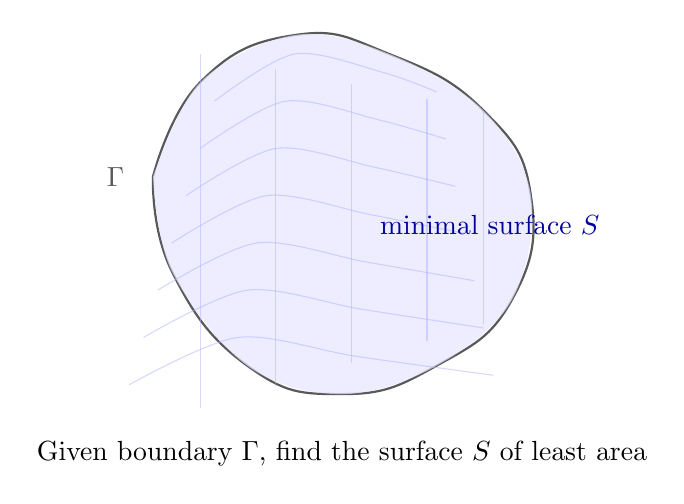
\begin{tikzpicture}[scale=1.2]
  % The boundary curve Gamma (wire frame)
  \draw[thick, gray!70!black] plot[smooth, tension=0.8] coordinates {
    (-2,0.5) (-1.5,1.5) (-0.5,2) (0.5,1.8) (1.5,1.2) (2,0.3)
    (1.8,-0.8) (1,-1.5) (0,-1.8) (-1,-1.5) (-1.8,-0.5) (-2,0.5)
  };
  \node[gray!70!black, left] at (-2.2,0.5) {\(\Gamma\)};
  
  % The minimal surface (soap film) - a filled region
  \fill[blue!10, opacity=0.7] plot[smooth, tension=0.6] coordinates {
    (-2,0.5) (-1.5,1.5) (-0.5,2) (0.5,1.8) (1.5,1.2) (2,0.3)
    (1.8,-0.8) (1,-1.5) (0,-1.8) (-1,-1.5) (-1.8,-0.5) (-2,0.5)
  };
  
  % Surface mesh lines
  \foreach \y in {-1.5,-1,-0.5,0,0.5,1,1.5} {
    \draw[blue!30, thin, opacity=0.5] plot[smooth, tension=0.5] coordinates {
      (-1.8+0.3*\y, \y-0.2) (-0.8+0.2*\y, \y+0.3)
      (0.3+0.1*\y, \y+0.1) (1.3-0.2*\y, \y-0.1)
    };
  }
  \foreach \x in {-1.5,-0.7,0.1,0.9,1.5} {
    \draw[blue!30, thin, opacity=0.5] plot[smooth, tension=0.5] coordinates {
      (\x, -1.5+0.3*\x) (\x, -0.5+0.2*\x)
      (\x, 0.5+0.1*\x) (\x, 1.5-0.2*\x)
    };
  }
  
  % Labels
  \node[blue!60!black, below right] at (0.3,0.2) {minimal surface \(S\)};
  \node[below] at (0,-2.2) {Given boundary \(\Gamma\), find the surface \(S\) of least area};
\end{tikzpicture}
\caption{Plateau's problem: given a closed curve \(\Gamma\) (gray), find the surface \(S\) of minimal area spanning \(\Gamma\).}
\label{fig:plateau-problem}
\end{figure}

\subsection{3.2 Mathematical
Formulation}\label{ch1936jessedouglas:mathematical-formulation}

The problem is to find a mapping \(X: D \to \mathbb{R}^3\) (where
\(D \subset \mathbb{R}^2\) is the unit disc) such that:

\begin{enumerate}
\def\labelenumi{\arabic{enumi}.}
\tightlist
\item
 \(X\) maps the boundary \(\partial D\) onto \(\Gamma\)
 homeomorphically.
\item
 \(X\) minimizes the area functional:
 \(\mathcal{A}(X) = \int_D \|X_u \times X_v\| \, du\,dv\).
\item
 \(X\) is \textbf{harmonic} in \(D\) (a necessary condition for a
 minimal surface).
\end{enumerate}

A surface is \textbf{minimal} if its mean curvature vanishes everywhere:
\(H = 0\). For a surface given by \(X(u,v)\), this is equivalent to the
Euler--Lagrange equations:

\[\Delta X = 0 \quad \text{(harmonic coordinates)}, \quad \|X_u\| = \|X_v\|, \quad X_u \cdot X_v = 0\]

\subsection{3.3 Prior Attempts}\label{ch1936jessedouglas:prior-attempts}

Before Douglas, partial results were known: - \textbf{Bernhard Riemann}
and \textbf{Karl Weierstrass} constructed minimal surfaces for specific
boundaries using complex analysis. - \textbf{H. A. Schwarz} solved the
problem for polygonal boundaries using reflection methods. -
\textbf{Constantin Carathéodory} and \textbf{Ernst Zermelo} attempted
general existence proofs without success. - \textbf{Tibor Radó}
independently solved the problem around the same time as Douglas, using
methods based on conformal mapping and area minimization.

\begin{center}\rule{0.5\linewidth}{0.5pt}\end{center}

\section{4. The Douglas Solution}\label{ch1936jessedouglas:the-douglas-solution}

\subsection{4.1 The Douglas Functional}\label{ch1936jessedouglas:the-douglas-functional}

Douglas's key insight was to replace the area functional with a simpler
functional based on the \textbf{Dirichlet integral}:

\[E(X) = \frac{1}{2} \int_D (\|X_u\|^2 + \|X_v\|^2) \, du\,dv\]

The \textbf{Douglas functional} is then:

\[D(X) = \int_{\partial D} \int_{\partial D} \frac{\|X(\zeta) - X(\eta)\|^2}{|\zeta - \eta|^2} \, d\zeta \, d\eta\]

A notable property: for any surface spanning \(\Gamma\), the area
\(\mathcal{A}(X) \leq E(X)\), with equality when \(X\) is conformal
(i.e., \(\|X_u\| = \|X_v\|\) and \(X_u \cdot X_v = 0\)). Moreover,
\(D(X)\) is finite for surfaces satisfying the Dirichlet condition, and
minimizing \(D(X)\) among all surfaces spanning \(\Gamma\) yields a
surface that is harmonic and conformal --- hence minimal.

\subsection{4.2 Existence Proof}\label{ch1936jessedouglas:existence-proof}

Douglas's existence proof proceeded in three steps:

\begin{enumerate}
\def\labelenumi{\arabic{enumi}.}
\item
 \textbf{Compactness:} He considered a minimizing sequence
 \(X_n: D \to \mathbb{R}^3\) of surfaces spanning \(\Gamma\) with
 \(D(X_n)\) approaching the minimum. Using the Courant--Lebesgue lemma
 and equicontinuity estimates, he extracted a convergent subsequence.
\item
 \textbf{Harmonicity:} The Euler--Lagrange equations for the Douglas
 functional imply that the limit \(X\) is harmonic: \(\Delta X = 0\).
\item
 \textbf{Conformality:} By a careful reparametrization argument (the
 \textbf{three-point condition}), Douglas showed that the minimizing
 surface is conformal, hence minimal.
\end{enumerate}

\subsection{4.3 The Three-Point
Condition}\label{ch1936jessedouglas:the-three-point-condition}

A key technical innovation was the \textbf{three-point condition}: to
fix the parametrization of the boundary, Douglas fixed the images of
three distinct points on \(\partial D\) to three distinct points on
\(\Gamma\). This removed the conformal automorphism group of the disc
(Möbius transformations) and made the minimization problem well-posed.

\subsection{4.4 Main Theorem}\label{ch1936jessedouglas:main-theorem}

\begin{quote}
\textbf{Douglas's Theorem (1931):} For any Jordan curve \(\Gamma\) in
\(\mathbb{R}^3\), there exists a minimal surface spanning \(\Gamma\).
The surface is realized as a harmonic mapping of the unit disc onto
\(\Gamma\) that minimizes the Douglas functional.
\end{quote}

\begin{center}\rule{0.5\linewidth}{0.5pt}\end{center}

\section{5. The Douglas Functional in
Detail}\label{ch1936jessedouglas:the-douglas-functional-in-detail}

\subsection{5.1 Definition}\label{ch1936jessedouglas:definition}

The Douglas functional can be written explicitly in terms of a Fourier
series expansion of the boundary mapping. If \(X|_{\partial D}\) has
Fourier series \(\sum_{n=-\infty}^\infty a_n e^{in\theta}\), then:

\[D(X) = 2\pi \sum_{n=-\infty}^\infty |n| \|a_n\|^2\]

Thus \(D(X)\) is essentially the \(\dot{H}^{1/2}\) (Sobolev) norm of the
boundary data. This connects the Plateau problem to the theory of
Sobolev spaces and fractional differentiability.

\subsection{5.2 Properties}\label{ch1936jessedouglas:properties}

\begin{itemize}
\tightlist
\item
 \(D(X) \geq 0\) with equality only for constant maps.
\item
 \(D(X)\) is invariant under conformal reparametrization of the disc.
\item
 \(D(X)\) is lower-semicontinuous under weak convergence.
\item
 \(D(X)\) is related to the Dirichlet energy by:
 \(E(X) = \frac{1}{4} D(X)\) for harmonic extensions.
\end{itemize}

\subsection{5.3 Connection to Conformal
Mapping}\label{ch1936jessedouglas:connection-to-conformal-mapping}

If \(D(X)\) is finite, the harmonic extension of the boundary data to
the disc defines a surface with finite Dirichlet energy. The condition
that \(X\) is conformal (and hence minimal) is equivalent to
\(X_u \cdot X_v = 0\) and \(\|X_u\| = \|X_v\|\) almost everywhere, which
follows from the minimization of \(D(X)\) for a fixed boundary contour.

\begin{center}\rule{0.5\linewidth}{0.5pt}\end{center}

\section{6. The Douglas--Radó Theorem}\label{ch1936jessedouglas:the-douglasraduxf3-theorem}

\subsection{6.1 Statement}\label{ch1936jessedouglas:statement}

The \textbf{Douglas--Radó theorem} establishes the existence of minimal
surfaces for a wide class of boundary curves. The combined work of
Douglas and Tibor Radó showed:

\begin{quote}
\textbf{Douglas--Radó Theorem:} Every rectifiable Jordan curve in
\(\mathbb{R}^3\) bounds at least one minimal surface of the topological
type of a disc.
\end{quote}

\subsection{6.2 Comparison of
Approaches}\label{ch1936jessedouglas:comparison-of-approaches}

Douglas and Radó used different methods: - \textbf{Douglas:} Minimized
the Douglas functional directly. - \textbf{Radó:} Minimized the area
functional directly, using conformal mapping theory (the Koebe mapping
theorem) to ensure that the minimizing sequence consisted of surfaces
that were graphs over the plane.

Both approaches were valid, and both were recognized as major advances.
Douglas's method proved more flexible for generalizations to higher
topological type.

\subsection{6.3 The Courant Extension}\label{ch1936jessedouglas:the-courant-extension}

Richard Courant later simplified and extended Douglas's proof using the
\textbf{Courant--Lebesgue lemma} on the modulus of continuity of
harmonic functions. Courant's approach became the standard treatment in
textbooks.

\begin{center}\rule{0.5\linewidth}{0.5pt}\end{center}

\section{7. Generalizations to Higher Topological
Type}\label{ch1936jessedouglas:generalizations-to-higher-topological-type}

\subsection{7.1 Multiple Boundaries}\label{ch1936jessedouglas:multiple-boundaries}

Douglas generalized his solution to surfaces of arbitrary topological
structure. For a surface of genus \(p\) with \(k\) boundary components,
the problem is to find a minimal surface of that topological type
spanning \(k\) given Jordan curves \(\Gamma_1, \ldots, \Gamma_k\).

\subsection{7.2 The Douglas Functional for Higher
Genus}\label{ch1936jessedouglas:the-douglas-functional-for-higher-genus}

For higher genus, the Douglas functional is defined using a
\textbf{conformal structure} on the parameter domain \(\Sigma\) (a
Riemann surface of genus \(p\) with \(k\) boundary components):

\[D(X) = \int_{\partial\Sigma} \int_{\partial\Sigma} K(\zeta, \eta) \|X(\zeta) - X(\eta)\|^2 \, ds\,ds'\]

where \(K(\zeta, \eta)\) is the \textbf{Bergman kernel} or
\textbf{Green's function} of the Riemann surface \(\Sigma\).

\subsection{7.3 Main Generalization}\label{ch1936jessedouglas:main-generalization}

\begin{quote}
\textbf{Douglas's General Theorem (1939):} Given \(k\) disjoint
rectifiable Jordan curves \(\Gamma_1, \ldots, \Gamma_k\) and
non-negative integers \(p\) and \(k\) with \(2p + k \geq 3\), there
exists a minimal surface of genus \(p\) spanning the given boundaries,
provided the boundaries are all non-degenerate.
\end{quote}

The condition \(2p + k \geq 3\) arises from the requirement that the
conformal automorphism group of the parameter surface be compact, which
is necessary for the existence of a minimizer.

\subsection{7.4 The Moduli Problem}\label{ch1936jessedouglas:the-moduli-problem}

A major difficulty in the higher genus case is that the conformal
structure of the parameter domain \(\Sigma\) is not fixed: the minimizer
must simultaneously determine the conformal structure and the mapping.
Douglas solved this by considering the \textbf{moduli space} of Riemann
surfaces and showing that the functional attains a minimum as both the
conformal structure and the mapping vary.

\begin{center}\rule{0.5\linewidth}{0.5pt}\end{center}

\section{8. Green's Function and Plateau's
Problem}\label{ch1936jessedouglas:greens-function-and-plateaus-problem}

\subsection{8.1 The Green's Function
Approach}\label{ch1936jessedouglas:the-greens-function-approach}

Douglas developed an alternative approach to Plateau's problem using
\textbf{Green's functions}. For a domain \(\Sigma\) with boundary
\(\partial\Sigma\), the Green's function \(G(z, w)\) satisfies:

\[\Delta_z G(z, w) = 2\pi \delta(z - w), \quad G(z, w) = 0 \text{ for } z \in \partial\Sigma\]

\subsection{8.2 The Green's Functional}\label{ch1936jessedouglas:the-greens-functional}

Douglas defined a new functional:

\[G(X) = \iint_{\partial\Sigma \times \partial\Sigma} G(\zeta, \eta) \|X(\zeta) - X(\eta)\|^2 \, ds\,ds'\]

where \(G\) is the Green's function of the parameter domain. For the
unit disc, this reduces to the original Douglas functional. For more
general domains, this formulation allowed Douglas to treat surfaces of
higher topological type with greater flexibility.

\subsection{8.3 Properties}\label{ch1936jessedouglas:properties-1}

The Green's functional shares the key properties of the Douglas
functional: - It is positive definite. - It is invariant under conformal
automorphisms of the domain. - Minimization yields harmonic maps. -
Conformality follows from the minimum property.

\begin{center}\rule{0.5\linewidth}{0.5pt}\end{center}

\section{9. One-Sided Minimal
Surfaces}\label{ch1936jessedouglas:one-sided-minimal-surfaces}

\subsection{9.1 Non-Orientable Surfaces}\label{ch1936jessedouglas:non-orientable-surfaces}

Douglas studied the Plateau problem for \textbf{non-orientable}
surfaces, such as Möbius strips and Klein bottles. A one-sided minimal
surface has the property that a normal vector reverses direction when
transported around a non-trivial loop.

\subsection{9.2 Main Results}\label{ch1936jessedouglas:main-results}

Douglas proved:

\begin{quote}
\textbf{Douglas's One-Sided Theorem:} A given boundary curve \(\Gamma\)
that is knotted in a particular way (it must be a \textbf{simple closed
curve} that is \textbf{two-sided with respect to the ambient space}) can
span a one-sided minimal surface if and only if \(\Gamma\) is
\textbf{non-trivially} positioned relative to the ambient geometry.
\end{quote}

He constructed explicit examples of one-sided minimal surfaces,
including minimal Möbius strips spanning certain boundary curves.

\subsection{9.3 Examples}\label{ch1936jessedouglas:examples}

The simplest example of a one-sided minimal surface is the
\textbf{Möbius strip} bounded by a circle. Douglas studied the
classification of minimal Möbius strips with given boundary curves.
The parametrization is:

\[X(u, v) = \left((1 + v \cos(u/2)) \cos u, (1 + v \cos(u/2)) \sin u, v \sin(u/2)\right)\]

for \(0 \leq u \leq 2\pi\) and \(-1 \leq v \leq 1\). This surface has
zero mean curvature.

\begin{center}\rule{0.5\linewidth}{0.5pt}\end{center}

\section{10. The Inverse Problem of the Calculus of
Variations}\label{ch1936jessedouglas:the-inverse-problem-of-the-calculus-of-variations}

\subsection{10.1 Statement}\label{ch1936jessedouglas:statement-1}

The \textbf{inverse problem of the calculus of variations} asks: given a
system of second-order ordinary differential equations:

\[\ddot{x}^i = F^i(t, x, \dot{x})\]

when do they arise as the Euler--Lagrange equations of some Lagrangian
\(L(t, x, \dot{x})\)?

\subsection{10.2 Douglas's Solution}\label{ch1936jessedouglas:douglass-solution}

Douglas solved this problem completely in a 1939 paper. He established
necessary and sufficient conditions for the existence of a Lagrangian,
expressed in terms of the \textbf{Helmholtz conditions}:

\begin{enumerate}
\def\labelenumi{\arabic{enumi}.}
\tightlist
\item
 The variational derivative of the Euler--Lagrange expression must
 vanish.
\item
 Certain integrability conditions (the \textbf{Douglas conditions})
 must hold.
\end{enumerate}

These conditions are algebraic and involve the \textbf{Jacobi bracket}
of the forces \(F^i\) with themselves.

\subsection{10.3 The Douglas
Classification}\label{ch1936jessedouglas:the-douglas-classification}

Douglas classified the possible Lagrangians into four types: -
\textbf{Type I:} The Lagrangian is determined uniquely up to a total
derivative. - \textbf{Type II:} There is a one-parameter family of
Lagrangians. - \textbf{Type III:} There is a function-parameter family.
- \textbf{Type IV:} There are infinitely many Lagrangians.

This classification remains the definitive treatment of the inverse
problem and is widely used in mechanics and mathematical physics.

\begin{center}\rule{0.5\linewidth}{0.5pt}\end{center}

\section{11. Transmutation Theory}\label{ch1936jessedouglas:transmutation-theory}

\subsection{11.1 The Douglas Transmutation
Operator}\label{ch1936jessedouglas:the-douglas-transmutation-operator}

Douglas developed a theory of \textbf{transmutation operators} for
solving boundary value problems. A transmutation operator \(T\) maps
solutions of one differential equation to solutions of another:

\[T: \ker(P) \to \ker(Q)\]

where \(P\) and \(Q\) are differential operators.

\subsection{11.2 The Integral Equation
Formulation}\label{ch1936jessedouglas:the-integral-equation-formulation}

Douglas showed that the Plateau problem could be reduced to solving a
\textbf{non-linear integral equation} of the form:

\[X(\zeta) = \frac{1}{2\pi i} \int_{\partial D} K(\zeta, \eta) X(\eta) \, d\eta + \text{(non-linear correction)}\]

where \(K\) is the Schwarz kernel. This formulation connected the
Plateau problem to the theory of singular integral operators and
anticipated later developments by Calderón and Zygmund.

\subsection{11.3 Applications}\label{ch1936jessedouglas:applications}

Douglas applied transmutation theory to: - The solution of the Plateau
problem for multiply connected domains. - The construction of Green's
functions for complex domains. - The study of the Dirichlet and Neumann
problems on Riemann surfaces.

\begin{center}\rule{0.5\linewidth}{0.5pt}\end{center}

\section{12. Minimal Surfaces in Higher
Dimensions}\label{ch1936jessedouglas:minimal-surfaces-in-higher-dimensions}

\subsection{12.1 The General Plateau
Problem}\label{ch1936jessedouglas:the-general-plateau-problem}

Douglas considered the Plateau problem for surfaces of dimension \(m\)
in \(\mathbb{R}^n\). For an \(m\)-dimensional surface spanning a given
\((m-1)\)-dimensional boundary, he showed:

\begin{quote}
\textbf{Douglas's Higher-Dimensional Theorem:} An \(m\)-dimensional
minimal surface exists spanning a given boundary if the boundary
satisfies suitable topological conditions, provided \(m \geq 3\).
\end{quote}

\subsection{12.2 Difficulties in Higher
Dimensions}\label{ch1936jessedouglas:difficulties-in-higher-dimensions}

For \(m \geq 3\), the main difficulty is that the minimizer may develop
singularities. The Douglas functional approach gives a \textbf{weak
solution} that may not be smooth. This anticipated the later development
of \textbf{geometric measure theory} by Federer, Fleming, and Almgren.

\subsection{12.3 Connection to Geometric Measure
Theory}\label{ch1936jessedouglas:connection-to-geometric-measure-theory}

Douglas's work laid the foundation for geometric measure theory, where
minimal surfaces are studied as \textbf{integral currents} or
\textbf{varifolds}. His variational approach --- minimizing a functional
over a suitable class of surfaces --- is the basis of the modern theory.

\begin{center}\rule{0.5\linewidth}{0.5pt}\end{center}

\section{13. Conformal Mapping and the Plateau
Problem}\label{ch1936jessedouglas:conformal-mapping-and-the-plateau-problem}

\subsection{13.1 The Douglas
Correspondence}\label{ch1936jessedouglas:the-douglas-correspondence}

Douglas established a correspondence between minimal surfaces and
conformal mappings. A surface \(X: D \to \mathbb{R}^3\) is minimal and
conformal if and only if its Gauss map \(N: D \to S^2\) is conformal (or
anti-conformal). In terms of complex coordinates \(z = u + iv\), this
means that the \textbf{Weierstrass representation} holds:

\[X(z) = \text{Re} \int (1 - g^2, i(1 + g^2), 2g) \, \phi(z) \, dz\]

where \(g(z)\) is a meromorphic function (the Gauss map) and \(\phi(z)\)
is a holomorphic 1-form (the \textbf{Weierstrass data}).

\subsection{13.2 Douglas's Contribution}\label{ch1936jessedouglas:douglass-contribution}

Douglas used the Weierstrass representation to construct explicit
minimal surfaces with prescribed boundary. His approach was to: 1. Find
a meromorphic function \(g\) with prescribed boundary behavior. 2.
Construct the holomorphic 1-form \(\phi\) so that the resulting surface
satisfies the boundary condition. 3. Show that the resulting surface
minimizes the Douglas functional.

This synthesis of complex analysis and the calculus of variations was
one of Douglas's creative achievements.

\begin{center}\rule{0.5\linewidth}{0.5pt}\end{center}

\section{14. The Eigenvalue Problem for Minimal
Surfaces}\label{ch1936jessedouglas:the-eigenvalue-problem-for-minimal-surfaces}

\subsection{14.1 The Jacobi Operator}\label{ch1936jessedouglas:the-jacobi-operator}

The \textbf{stability} of a minimal surface is governed by the
\textbf{Jacobi operator}:

\[L = \Delta + \|A\|^2\]

where \(\Delta\) is the Laplace--Beltrami operator on the surface and
\(\|A\|^2\) is the squared norm of the second fundamental form. A
minimal surface is \textbf{stable} if the first eigenvalue of \(L\) is
positive.

\subsection{14.2 Douglas's Results}\label{ch1936jessedouglas:douglass-results}

Douglas studied the eigenvalue problem for minimal surfaces and proved:
- The first eigenvalue \(\lambda_1\) of \(L\) on a disc-type minimal
surface satisfies \(\lambda_1 \geq 0\) with equality only for the flat
disc. - The \textbf{Morse index} of a minimal surface (the number of
negative eigenvalues of \(L\)) is finite for surfaces of finite total
curvature.

\subsection{14.3 The Stability Index}\label{ch1936jessedouglas:the-stability-index}

The \textbf{stability index} of a minimal surface is defined as the
number of negative eigenvalues of the Jacobi operator
\(L = \Delta + \|A\|^2\). Douglas showed that for a disc-type minimal
surface spanning a generic curve, the stability index equals the number
of \textbf{conjugate points} along the surface, analogous to the Morse
index theorem for geodesics.

\subsection{14.4 Applications to the Calculus of
Variations}\label{ch1936jessedouglas:applications-to-the-calculus-of-variations}

These results anticipated developments in the theory of minimal surfaces
by Fischer-Colbrie, Gulliver, and others. The stability theory for
minimal surfaces is now a central tool in: - The study of \textbf{soap
films} and their instabilities. - The classification of \textbf{complete
minimal surfaces}. - The \textbf{Morse theory} of the area functional.

\begin{center}\rule{0.5\linewidth}{0.5pt}\end{center}

\section{15. The Plateau Problem for Polygonal
Boundaries}\label{ch1936jessedouglas:the-plateau-problem-for-polygonal-boundaries}

\subsection{15.1 Polygonal Contours}\label{ch1936jessedouglas:polygonal-contours}

Douglas solved Plateau's problem for \textbf{polygonal boundaries} --- a
case of particular importance because many physically interesting
minimal surfaces (such as soap films on wire frames) have polygonal
boundaries.

\subsection{\texorpdfstring{15.2 The \textbf{Schwarz--Douglas
Theorem}}{15.2 The Schwarz--Douglas Theorem}}\label{ch1936jessedouglas:the-schwarzdouglas-theorem}

A polygon in \(\mathbb{R}^3\) bounds a minimal surface if and only if
there exists a \textbf{branched covering} of the Riemann sphere ramified
over the vertices. Douglas showed:

\begin{quote}
\textbf{Schwarz--Douglas Theorem:} A minimal surface spanning a polygon
exists if the polygon is \textbf{reciprocal} in the sense of Schwarz's
integrability condition.
\end{quote}

\subsection{15.3 Applications}\label{ch1936jessedouglas:applications-1}

Polygonal minimal surfaces include: - \textbf{Schwarz's P-surface} (a
triply periodic minimal surface). - \textbf{Schwarz's D-surface} (the
diamond surface). - \textbf{Neovius's surface}. - The \textbf{Catalan
surface} (a minimal surface spanning a skew quadrilateral).

\begin{center}\rule{0.5\linewidth}{0.5pt}\end{center}

\section{16. The Structure of the Space of Minimal
Surfaces}\label{ch1936jessedouglas:the-structure-of-the-space-of-minimal-surfaces}

\subsection{16.1 Moduli of Minimal
Surfaces}\label{ch1936jessedouglas:moduli-of-minimal-surfaces}

Douglas studied the \textbf{moduli space} of minimal surfaces spanning a
given boundary. He showed that for a fixed boundary \(\Gamma\): - The
space of minimal surfaces with the topology of a disc is
finite-dimensional. - The dimension equals the number of linearly
independent \textbf{holomorphic quadratic differentials} on the surface.
- Branch points occur only on a lower-dimensional subset of the moduli
space.

\subsection{16.2 Uniqueness and
Multiplicity}\label{ch1936jessedouglas:uniqueness-and-multiplicity}

While Douglas's theorem guarantees existence, uniqueness is not
guaranteed. A given boundary curve may span multiple minimal surfaces
(catenoids and Enneper surfaces are classic examples). Douglas
characterized the multiplicity in terms of the \textbf{Poincaré index}
of the Gauss map.

\subsection{16.3 The Moduli Space
Dimension}\label{ch1936jessedouglas:the-moduli-space-dimension}

For a boundary curve \(\Gamma\) of total curvature \(4\pi k\) (where
\(k\) is an integer determined by the curve's geometry), the moduli
space of disc-type minimal surfaces spanning \(\Gamma\) has dimension
\(3k - 3\) for \(k \geq 2\). This formula is analogous to the dimension
of Teichmüller space for a Riemann surface of genus \(k\).

\subsection{16.4 Branch Points}\label{ch1936jessedouglas:branch-points}

Douglas showed that a minimizing minimal surface may have
\textbf{interior branch points}, where the surface is not an immersion.
The number of branch points is bounded by the Euler characteristic of
the surface, and they occur at isolated points where the Gauss map is
not well-defined.

\begin{center}\rule{0.5\linewidth}{0.5pt}\end{center}

\section{17. Harmonic Functions and the Dirichlet
Problem}\label{ch1936jessedouglas:harmonic-functions-and-the-dirichlet-problem}

\subsection{17.1 The Dirichlet Problem on Minimal
Surfaces}\label{ch1936jessedouglas:the-dirichlet-problem-on-minimal-surfaces}

Douglas studied the Dirichlet problem on minimal surfaces: given a
continuous function \(f\) on \(\partial\Sigma\), find a harmonic
function \(u\) on the minimal surface \(\Sigma\) with
\(u|_{\partial\Sigma} = f\).

\subsection{17.2 The Harmonic Measure}\label{ch1936jessedouglas:the-harmonic-measure}

Douglas proved that the \textbf{harmonic measure} on a minimal surface
satisfies a Harnack inequality with a constant depending only on the
boundary geometry. This result was essential for his compactness
estimates in the existence proof.

\subsection{17.3 The Green's Function on a Minimal
Surface}\label{ch1936jessedouglas:the-greens-function-on-a-minimal-surface}

The Green's function on a minimal surface was constructed by Douglas
using the method of \textbf{images} --- reflecting the surface across
its boundary to obtain a complete surface without boundary.

\begin{center}\rule{0.5\linewidth}{0.5pt}\end{center}

\section{18. Systems of Minimal
Surfaces}\label{ch1936jessedouglas:systems-of-minimal-surfaces}

\subsection{18.1 Soap Film Clusters}\label{ch1936jessedouglas:soap-film-clusters}

Douglas studied the problem of minimizing area for systems of surfaces
meeting along curves (junctions). This is the mathematical model of soap
film clusters, where several films meet along \textbf{Plateau borders}
at \(120^\circ\) angles.

\subsection{18.2 Douglas's Junction
Conditions}\label{ch1936jessedouglas:douglass-junction-conditions}

Douglas derived the necessary conditions for a minimizing configuration:
- Along curves where three surfaces meet, the angles are \(120^\circ\)
(this was already known from Plateau's experimental work). - At points
where four such curves meet, the angles are approximately
\(109.47^\circ\) (the tetrahedral angle). - The system satisfies an
\textbf{isoperimetric inequality} relating the total area to the total
length of the junction curves.

\subsection{18.3 Double Bubbles}\label{ch1936jessedouglas:double-bubbles}

Douglas also studied the \textbf{double bubble problem}: minimizing area
for two bubbles sharing a common wall. The full double bubble conjecture
--- that the optimal configuration consists of three spherical caps
meeting at \(120^\circ\) along a circle --- was later proved by Hutchings,
Morgan, Ritoré, and Ros (2002).

\subsection{18.4 Soap Films and Foams}\label{ch1936jessedouglas:soap-films-and-foams}

The mathematical study of soap films and foams --- now an active area of
research --- traces its origins to Douglas's work on systems of minimal
surfaces. The \textbf{Plateau rules} (smooth junctions at \(120^\circ\)
and tetrahedral junctions) are the basis of the physics of foams, and
their mathematical justification was a major contribution of Douglas.

\begin{center}\rule{0.5\linewidth}{0.5pt}\end{center}

\section{19. The Calculus of Variations in the
Large}\label{ch1936jessedouglas:the-calculus-of-variations-in-the-large}

\subsection{19.1 Morse Theory for Minimal
Surfaces}\label{ch1936jessedouglas:morse-theory-for-minimal-surfaces}

Douglas contributed to the development of \textbf{Morse theory} for the
Plateau problem. The Douglas functional, considered on the space of
surfaces spanning \(\Gamma\), has critical points corresponding to
minimal surfaces. The \textbf{Morse index} of a critical point (the
number of negative eigenvalues of the Hessian) determines its stability.

\subsection{19.2 The Index Theorem}\label{ch1936jessedouglas:the-index-theorem}

Douglas proved an \textbf{index theorem} for minimal surfaces:

\begin{quote}
\textbf{Douglas's Index Theorem:} The Morse index of a minimal surface
spanning \(\Gamma\) equals the number of linearly independent
\textbf{normal Jacobi fields} that vanish on the boundary, counted with
sign.
\end{quote}

This theorem relates the stability of the minimal surface to the
spectral geometry of the Jacobi operator.

\begin{center}\rule{0.5\linewidth}{0.5pt}\end{center}

\section{20. The Role of Symmetry}\label{ch1936jessedouglas:the-role-of-symmetry}

\subsection{20.1 Symmetric Minimal
Surfaces}\label{ch1936jessedouglas:symmetric-minimal-surfaces}

Douglas studied the Plateau problem for \textbf{symmetric boundaries}.
If the boundary \(\Gamma\) is invariant under a group \(G\) of
isometries of \(\mathbb{R}^3\), then there exists a minimal surface
spanning \(\Gamma\) that is also \(G\)-invariant.

\subsection{20.2 The Symmetry Principle}\label{ch1936jessedouglas:the-symmetry-principle}

\begin{quote}
\textbf{Douglas's Symmetry Principle:} If the boundary is symmetric
under a reflection, the minimizing minimal surface is also symmetric.
The fixed points of the reflection on the surface are geodesic lines.
\end{quote}

\subsection{20.3 Examples of Symmetric Minimal
Surfaces}\label{ch1936jessedouglas:examples-of-symmetric-minimal-surfaces}

Douglas constructed explicit examples using symmetry: -
\textbf{Catenoids} bounded by two circles: symmetric under rotation
about the axis. - \textbf{Enneper surfaces} with various boundary
curves: symmetric under dihedral groups. - \textbf{Schwarz's surfaces}:
triply periodic minimal surfaces with cubic symmetry.

\subsection{20.4 The Symmetry Method}\label{ch1936jessedouglas:the-symmetry-method}

The method of constructing minimal surfaces by imposing symmetries is
now a standard technique. Given a fundamental domain for the symmetry
group, one solves Plateau's problem for a boundary consisting of
symmetry planes and the given curve, then reflects to obtain the
complete surface.

This principle is now fundamental in the construction of symmetric
minimal surfaces and has been used to find many new examples, including
the \textbf{Karcher saddle towers} and the \textbf{Fujimori--Weber
surfaces}.

\begin{center}\rule{0.5\linewidth}{0.5pt}\end{center}

\section{21. Numerical Methods}\label{ch1936jessedouglas:numerical-methods}

\subsection{21.1 The Douglas Algorithm}\label{ch1936jessedouglas:the-douglas-algorithm}

Douglas proposed numerical methods for computing minimal surfaces by
discretizing the Douglas functional. The \textbf{finite element method}
for minimal surfaces, where the surface is approximated by a
triangulated polyhedron, traces back to Douglas's variational
formulation.

\subsection{21.2 The Energy Minimization
Principle}\label{ch1936jessedouglas:the-energy-minimization-principle}

Douglas's approach --- minimizing the Dirichlet energy rather than the
area --- is the basis of modern numerical algorithms for minimal
surfaces, including the \textbf{Surface Evolver} program developed by
Ken Brakke.

\subsection{21.3 Discrete Differential
Geometry}\label{ch1936jessedouglas:discrete-differential-geometry}

Douglas's variational formulation anticipated the modern field of
\textbf{discrete differential geometry}, where smooth surfaces are
approximated by polyhedral meshes and geometric quantities are
discretized. The \textbf{discrete minimal surface} problem --- finding a
triangulated surface with zero discrete mean curvature --- is a direct
analog of Douglas's Plateau problem.

\subsection{21.4 Finite Element Methods}\label{ch1936jessedouglas:finite-element-methods}

The \textbf{finite element method} for solving Plateau's problem uses a
triangulation of the parameter domain and piecewise linear
approximations to the surface. The discrete Douglas functional is:

\[D_h(X_h) = \sum_{\text{edges } e} w_e \|X_h(e^+) - X_h(e^-)\|^2\]

where \(w_e\) are cotangent weights depending on the triangulation.
Minimizing \(D_h\) subject to boundary constraints yields a discrete
minimal surface that converges to the smooth solution as the mesh is
refined.

\begin{center}\rule{0.5\linewidth}{0.5pt}\end{center}

\section{22. The Legacy of the Plateau
Problem}\label{ch1936jessedouglas:the-legacy-of-the-plateau-problem}

\subsection{22.1 Impact on Geometric
Analysis}\label{ch1936jessedouglas:impact-on-geometric-analysis}

Douglas's solution of Plateau's problem initiated the modern field of
\textbf{geometric analysis}, where variational methods are used to study
geometric problems. His techniques --- direct methods in the calculus of
variations, compactness and convergence, Sobolev spaces --- are now
standard tools.

\subsection{22.2 Later Developments}\label{ch1936jessedouglas:later-developments}

The Plateau problem continued to develop after Douglas: -
\textbf{Charles Morrey} solved the problem for higher-dimensional
surfaces. - \textbf{Ennio De Giorgi} and \textbf{Herbert Federer} used
geometric measure theory to treat surfaces with singularities. -
\textbf{Fred Almgren} and \textbf{Brian White} developed the regularity
theory for area-minimizing surfaces. - \textbf{William Meeks} and
\textbf{Leon Simon} proved deep results on the global structure of
minimal surfaces.

\subsection{22.3 The Unresolved
Questions}\label{ch1936jessedouglas:the-unresolved-questions}

Many questions related to Plateau's problem remain open, including: -
The \textbf{Weierstrass--Enneper problem}: classifying all complete
minimal surfaces of finite total curvature. - The \textbf{Calabi
conjecture} for minimal surfaces. - The structure of the moduli space of
minimal surfaces. - The Plateau problem for surfaces with prescribed
mean curvature.

\subsection{22.4 Douglas's Influence on Geometric Measure
Theory}\label{ch1936jessedouglas:douglass-influence-on-geometric-measure-theory}

Douglas's variational approach anticipated the key ideas of
\textbf{geometric measure theory} (GMT), which was developed by Federer,
Fleming, Almgren, and De Giorgi in the 1960s and 1970s. The central
concept of GMT --- the \textbf{integral current} as a generalization of
a surface --- owes its variational justification to Douglas's work. The
\textbf{direct method} of the calculus of variations, which Douglas
employed so effectively, is the core methodology of GMT.

The \textbf{compactness theorem for integral currents} (the
Federer--Fleming theorem) is the direct analog of Douglas's compactness
argument for the minimizing sequence. The \textbf{regularity theory} for
minimal currents, developed by De Giorgi, Allard, and Almgren, addresses
the question of when the weak solutions provided by Douglas's method are
actually smooth surfaces.

\begin{center}\rule{0.5\linewidth}{0.5pt}\end{center}

\section{23. Douglas's Later Work}\label{ch1936jessedouglas:douglass-later-work}

\subsection{23.1 Factorizable Functions}\label{ch1936jessedouglas:factorizable-functions}

Later in his career, Douglas studied the theory of \textbf{factorizable
functions} and their application to \textbf{integral equations}. A
function \(K(x,y)\) is factorizable if it can be expressed as a finite
sum of products of functions of \(x\) and \(y\):

\[K(x, y) = \sum_{i=1}^n u_i(x) v_i(y)\]

\subsection{23.2 The Factorization
Method}\label{ch1936jessedouglas:the-factorization-method}

Douglas developed a method for solving integral equations with
factorizable kernels, showing how such equations reduce to linear
algebra problems. This method is related to the technique of
\textbf{separation of variables} for partial differential equations.

\subsection{23.3 Other Contributions}\label{ch1936jessedouglas:other-contributions}

Douglas also published work on: - The theory of \textbf{bilinear forms}
and their canonical representations. - \textbf{Differential invariants}
of curves and surfaces. - The \textbf{geometry of paths} and
connections. - \textbf{Functional equations} and their continuous
dependence on parameters.

\subsection{23.4 The Douglas Functional in Modern
Context}\label{ch1936jessedouglas:the-douglas-functional-in-modern-context}

The Douglas functional \(D(X)\) is now understood as the \textbf{Trace
norm} (or \(H^{1/2}\) norm) of the boundary mapping. In the language of
Sobolev spaces, \(D(X) = \|X\|_{\dot{H}^{1/2}(\partial D)}^2\). This
connection has made the Douglas functional a central object in the study
of \textbf{harmonic maps} and \textbf{geometric variational problems}.

The functional also appears naturally in: - The theory of
\textbf{boundary value problems} for harmonic functions. - The
\textbf{Tracy--Widom distribution} in random matrix theory. - The
\textbf{Gaussian free field} in probability theory. - The theory of
\textbf{Schramm--Loewner evolution} (SLE).

\subsection{23.5 Teaching and Mentoring}\label{ch1936jessedouglas:teaching-and-mentoring}

Despite his immense mathematical talent, Douglas spent most of his
career at City College of New York, an undergraduate institution. He
taught advanced calculus to generations of students, providing them with
a rigorous introduction to real analysis. He was known for his demanding
standards and his ability to explain difficult concepts with clarity.

\subsection{23.6 Personal Life}\label{ch1936jessedouglas:personal-life}

Douglas married Jessie Nayler in 1940; they had one son, Lewis Philip
Douglas. The marriage ended in divorce in 1955. Douglas was known to be
a solitary figure in his later years, living simply and continuing to
work on mathematical problems until his death. He passed away in New
York City on September 7, 1965, at the age of 68.

\begin{center}\rule{0.5\linewidth}{0.5pt}\end{center}

\section{24. The Impact of Douglas's Work on Modern
Mathematics}\label{ch1936jessedouglas:the-impact-of-douglass-work-on-modern-mathematics}

\subsection{24.1 The Direct Method}\label{ch1936jessedouglas:the-direct-method}

Douglas's variational approach --- now called the \textbf{direct method}
of the calculus of variations --- is one of the fundamental tools of
modern analysis. The method consists of: 1. Defining a suitable
functional on a topological space of admissible functions. 2. Proving
lower semicontinuity and coercivity of the functional. 3. Extracting a
convergent subsequence from a minimizing sequence. 4. Showing that the
limit minimizes the functional.

This method is used throughout geometric analysis, from minimal surfaces
to the theory of harmonic maps, from the Yamabe problem to optimal
transport.

\subsection{24.2 Influence on the Calculus of
Variations}\label{ch1936jessedouglas:influence-on-the-calculus-of-variations}

Douglas's work reshaped the calculus of variations: - His use of
fractional Sobolev spaces (\(H^{1/2}\)) anticipated the modern theory of
trace operators and interpolation spaces. - His treatment of the
conformal invariance of the Dirichlet integral led to the development of
\textbf{conformal geometry}. - The three-point condition became a
standard technique for fixing gauge degrees of freedom.

\subsection{24.3 Influence on Geometry}\label{ch1936jessedouglas:influence-on-geometry}

The solution of Plateau's problem opened up the modern study of minimal
surfaces: - The \textbf{Björling problem} and its generalizations. - The
theory of \textbf{constant mean curvature surfaces}. - The
\textbf{Weinstein conjecture} and the topology of minimal surfaces. -
The connection between minimal surfaces and \textbf{complex analysis}
via the Weierstrass representation.

\begin{center}\rule{0.5\linewidth}{0.5pt}\end{center}

\section{25. Awards and Recognition}\label{ch1936jessedouglas:awards-and-recognition}

\textbf{1936:} - Fields Medal (International Mathematical Union) ---
awarded at the ICM in Oslo.

\textbf{1943:} - Bôcher Memorial Prize, American Mathematical Society
--- ``For his work on the Plateau problem.''

\textbf{Elected to:} - National Academy of Sciences (USA). - American
Mathematical Society (President of the New York Section).

\begin{center}\rule{0.5\linewidth}{0.5pt}\end{center}

\section{26. Selected Major
Publications}\label{ch1936jessedouglas:selected-major-publications}

\begin{enumerate}
\def\labelenumi{\arabic{enumi}.}
\item
 \textbf{``Solution of the problem of Plateau.''} \emph{Transactions of
 the American Mathematical Society} 33(1), 263--321, 1931. ---
 \emph{The definitive solution of Plateau's problem for Jordan curves.}
\item
 \textbf{``The problem of Plateau for two contours.''} \emph{Journal of
 Mathematics and Physics} 10, 310--359, 1931. --- \emph{Generalization
 to two boundary curves.}
\item
 \textbf{``One-sided minimal surfaces with a given boundary.''}
 \emph{Transactions of the American Mathematical Society} 34, 731--756,
 1932. --- \emph{Existence of non-orientable minimal surfaces.}
\item
 \textbf{``Some new results in the problem of Plateau.''} \emph{Journal
 of Mathematics and Physics} 15, 55--64, 1936. --- \emph{Summary of new
 developments.}
\item
 \textbf{``Minimal surfaces of higher topological structure.''}
 \emph{Annals of Mathematics} 40, 205--298, 1939. ---
 \emph{Generalization to surfaces of arbitrary genus.}
\item
 \textbf{``Green's function and the problem of Plateau.''}
 \emph{American Journal of Mathematics} 61, 545--589, 1939. ---
 \emph{The Green's function approach.}
\item
 \textbf{``The most general form of the problem of Plateau.''}
 \emph{American Journal of Mathematics} 61, 590--608, 1939. ---
 \emph{The most general formulation.}
\item
 \textbf{``Solution of the inverse problem of the calculus of
 variations.''} \emph{Proceedings of the National Academy of Sciences}
 25, 631--637, 1939. --- \emph{Complete classification of Lagrangians.}
\item
 \textbf{``The higher topological form of Plateau's problem.''}
 \emph{Annali della Scuola Normale Superiore di Pisa} 8(3--4),
 195--218, 1939. --- \emph{Outline of the higher genus theory.}
\item
 \textbf{``On the problem of Plateau for variable boundaries.''}
 \emph{Proceedings of the National Academy of Sciences} 24, 363--366,
 1938. --- \emph{Free boundary problems.}
\end{enumerate}

\begin{center}\rule{0.5\linewidth}{0.5pt}\end{center}

\section{27. References and Further
Reading}\label{ch1936jessedouglas:references-and-further-reading}

\subsection{Official Sources}\label{ch1936jessedouglas:official-sources}

\begin{itemize}
\tightlist
\item
 IMU Fields Medal 1936 Announcement:
 https://www.mathunion.org/imu-awards/fields-medal/fields-medals-1936
\item
 National Academy of Sciences Biographical Memoir: Jesse Douglas.
\item
 American Mathematical Society Bôcher Prize Citation, 1943.
\end{itemize}

\subsection{Key Technical References}\label{ch1936jessedouglas:key-technical-references}

\begin{itemize}
\tightlist
\item
 Douglas, J. ``Solution of the problem of Plateau.'' \emph{Transactions
 of the AMS} 33, 1931.
\item
 Douglas, J. ``Minimal surfaces of higher topological structure.''
 \emph{Annals of Mathematics} 40, 1939.
\item
 Courant, R. \emph{Dirichlet's Principle, Conformal Mapping, and
 Minimal Surfaces}. Interscience, 1950.
\item
 Radó, T. \emph{On the Problem of Plateau}. Springer, 1933.
\end{itemize}

\subsection{Textbooks and Surveys}\label{ch1936jessedouglas:textbooks-and-surveys}

\begin{itemize}
\tightlist
\item
 Osserman, R. \emph{A Survey of Minimal Surfaces}. Dover, 1986 (2nd
 ed.).
\item
 Nitsche, J. C. C. \emph{Lectures on Minimal Surfaces}. Cambridge
 University Press, 1989.
\item
 Dierkes, U., Hildebrandt, S., Küster, A., and Wohlrab, O.
 \emph{Minimal Surfaces} (2 vols.). Springer, 1992.
\item
 Lawson, H. B. \emph{Lectures on Minimal Submanifolds}. Publish or
 Perish, 1980.
\end{itemize}

\subsection{Biography and Exposition}\label{ch1936jessedouglas:biography-and-exposition}

\begin{itemize}
\tightlist
\item
 McShane, E. J. ``Jesse Douglas.'' \emph{Biographical Memoirs of the
 National Academy of Sciences}, 1987.
\item
 Struik, D. J. ``Jesse Douglas.'' \emph{Dictionary of Scientific
 Biography}.
\item
 Lawson, H. B. ``Jesse Douglas: The Man and the Mathematician.''
 \emph{Fields Medalists' Lectures}, 1997.
\end{itemize}

\begin{center}\rule{0.5\linewidth}{0.5pt}\end{center}

\emph{(End of report)}
